% !TEX root = Dokumentation_SysSpec.tex
\subsection{Externe Schnittstellen}
\subsubsection{Rollen und Akteure}
Im Rahmen des Filial-Bestellsystems existieren folgende Akteure, welche zugleich spezifische Rollen und somit Berechtigungen besitzen.
\begin{itemize}
	\item Benutzer: Jeder Akteur in der Rolle 'Benutzer' kann sich am System mit den entsprechenden Zugangsdaten anmelden.
	\item Filialleiter: besitzt die Rechte 'OrderView' und 'OrderEdit' und kann daher sowohl bestehende Bestellungen einsehen, bearbeiten und annullieren.
	\item Verkaufspersonal: hat grundsätzlich identische Rechte wie Filialleiter, kann jedoch zusätzlich noch Bestellungen erfassen. TODO: Prüfen, ob wirklich so umgesetzt!
	\item Datentypist: besitzt die Rolle 'Supply' und kann dadurch den Wareneingang im System erfassen
	\item Filialverwalter: besitzt die Rolle 'LogView' und kann daher das Logfile mit den abgelaufenen Systemabläufen überprüfen. Die Einsicht via Filial-Bestellsystem in das Logfile ist nicht im Release 1.0 realisiert. In folgenden Releases wird über eine zentrale Logfile-Verwaltung (bspw. Syslog) entschieden. 
	\item Sysadmin: hat keine aktiven Steuerungsmöglichkeiten innerhalb des Systems. Der Anwendungsfall des Sysadmins ist für Release 1.0 noch nicht definiert.
\end{itemize}
\subsubsection{Datenbankanbindung}
TODO Tobias: OR-Mapper Anbindung beschreiben\\

Für die Persistierung der Daten (ausser Logdaten, RW und Zentrallager) wird eine MySQL-Datenbank aus dem EnterpriseLab mit dem folgenden ConnectionString verwendet:
- TODO ConnectionString
Auf Stufe Datenbank wurden keine weiteren Sichten, Prozeduren und Benutzer eingesetzt. Daher wird gegenüber der Datenbank nur der User grp13 verwendet.
\subsubsection{Zentrallager}
Für das Zentrallager wird eine Stock-Schnittstelle zur Verfügung gestellt. Sie ist in einem Maven-Repo ('https://bintray.com/hslu/maven/appe/5.0.1\#files/ch/hslu/appe/appe\_stock') abgelegt und bereits in das Modul 'appe\_layer\_business' integriert.\\
Die detaillierte Dokumentation zur vorgegebenen Schnittstelle ist unter\\
'https://elearning.hslu.ch/ilias/ilias.php?ref\_id=3290529\&page=APPE\_Startseite\&wpg\_id=11071\&cmd=downloadFile\&cmdClass=ilwikipagegui\&cmdNode=yi:l5:yk\&baseClass=ilwikihandlergui\&file\_id=il\_\_file\_3582976' zu beziehen.

Die Implementation wurde im Business-Layer vorgenommen. Die vorgegebene Schnittstelle wurde nur in einem minimalen Ausmass verwendet. Im Rahmen einer Bestelländerung /-erfassung wird bei Unterschreiten der definierten Mindestanzahl eines Artikels (bis Release 1.0 fix auf 2 definiert) über die Methode 'orderArticle(....)' eine Nachbestellung in der Höhe der geforderten Artikel + 2 ausgelöst. Es wird dabei nicht geprüft, ob am Zentrallager noch entsprechende Artikel vorhanden sind. \\Es wird daher davon ausgegangen, dass am Zentrallager wie auch im Filiallager ein Negativlagerbestand möglich ist. Die Schnittstelle ist dadurch nur unidirektional und es werden keine Daten \& Interaktionen durch das Zentrallager an das Filial-Bestellsystem direkt ausgeführt.  \\
TODO Severin: Klassendiagram hinzufügen
\subsubsection{Rechnungswesen}
Das Rechnungswesen hat die Aufgabe bei Erfassung / Änderung einer Bestellung eine entsprechende Rechnung an den Kunden zu versenden.\\
Von Seiten Auftraggeber sind keine Schnittstellen zur Verfügung gestellt worden und daher wurden die entsprechenden Aufgaben des Rechnungswesen als simpler Stub implementiert, der lediglich ein Output über die ausgeführte Arbeit (z.B. Neue Rechnung gedruckt) protokolliert. \\
TODO Severin: Klassendiagram hinzufügen

\subsection{Interne Schnittstellen}
In diesem Kapitel werden nur wichtige, systemrelevante Schnittstellen spezifiziert. Es werden primär die Schnittstellen zwischen den Layern 'Client', 'Business' inkl. Remote und 'Data' beschrieben.

\subsubsection{Globale Sicht}
In einer groben Übersicht wird die globale Sicht der Schnittstellen zwischen den Schichten / Packages aufgezeigt.:\\
\begin{figure}[H]
\centering
	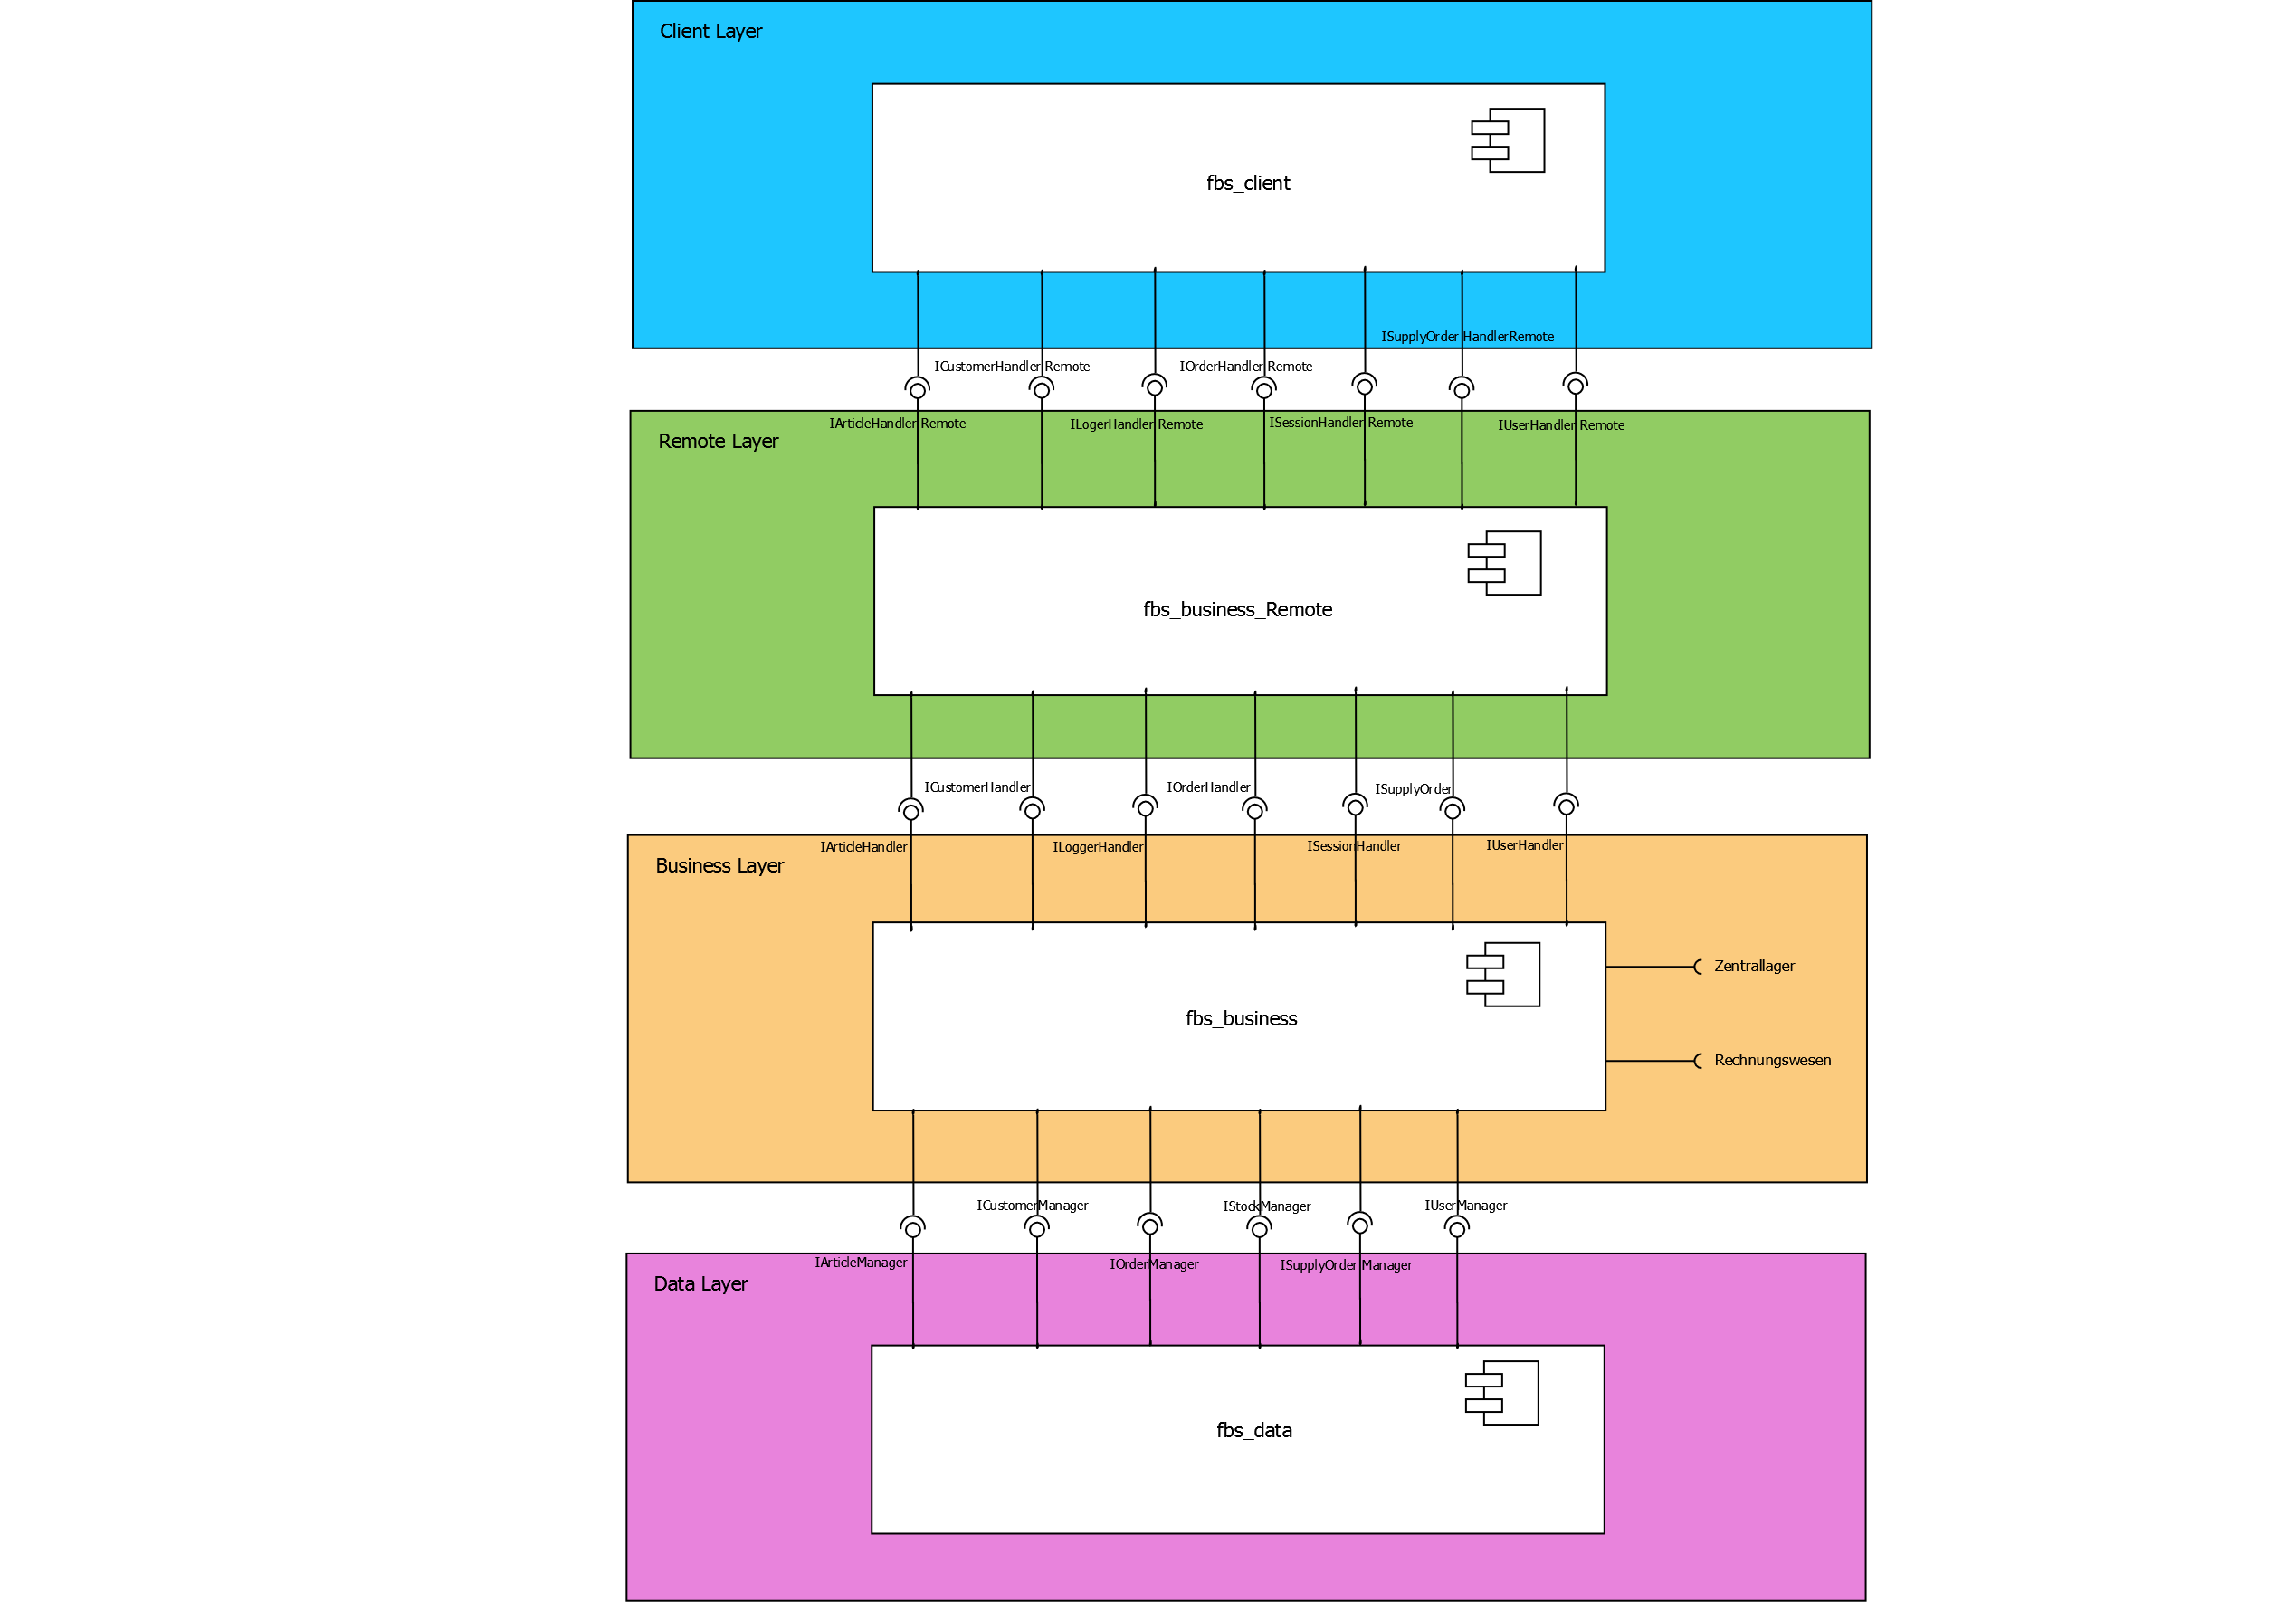
\includegraphics[width=1.0\linewidth]{Images/Schnittstellen}
	\caption{Schnittstellen}
	\label{fig:schnittstellen}
\end{figure}

\subsubsection{Model}
TODO Severin Schnittstellen zu Business oder was ist hier gemeint?

\subsubsection{Client <-> Business-Remote}
Der Client-Layer ist generell als MVC implementiert. Der Controller fordert bei Aktionen des Benutzers jeweils die nachgefragten Informationen über die Remote-Schicht an, und sendet neue und geänderte Bestellungen über die definierten Schnittstellen zur Remote-Schicht.
Der Client-Layer strukturiert die erhaltenen Daten in einem eigenen Model transient ab.
TODO Klassendiagramme hinzufügen, eventuell Sequenz-Diagram

Speziell ist das User- und Session-Management. Der User erhält auf Basis der über die Login-Schnittstelle erhaltenen Benutzergruppe seine Berechigung zugewiesen. Diese Zuweisung wird im Singelton-Pattern des Users abgespeichert.
Das Singleton-Pattern wird dabei benötigt, um den Kontext des Benutzers auf Business-Ebene zu prüfen.
TODO Klassendiagram hinzufügen

Die Kontext-Prüfung wird dabei über eine dedizierte Schnittstelle zu Beginn jedes Aufrufes eingeleitet. So werden ungültige Aufrufe verhindert.
TODO Klassendiagramme Hnzufügen

Der Login-Prozess der Applikation entscheidet auf Basis der erhaltenen Benutzergruppe, welche Ansicht der jeweilige Benutzer erhält. Diese Entscheidung ist dabei über ein Strategy-Pattern implementiert. 
TODO Klassendiagramme Hnzufügen

Die Implementation des Client-Layers beruht auf JavaFX, bzw. FXML. Diese Implementation erzwingt den Einsatz von Observable-Objekten.

Der Client ist stark von der Remote-Schicht der Business-Logik abhängig. Es ist nicht gedacht, dass der Client-Layer für andere Applikationen verwendet wird.


\subsubsection{Business-Remote <-> Business-Core}
TODO Marco
\subsubsection{Business-Core <-> Data}
TODO Marco \&Tobias
